% !TeX program = pdflatex
\documentclass[11pt,a4paper]{article}
\usepackage[utf8]{inputenc}
\usepackage[T1]{fontenc}
\usepackage[turkish]{babel}
\usepackage{lmodern}
\usepackage{geometry}
\usepackage{graphicx}
\usepackage{caption}
\usepackage{subcaption}
\usepackage{booktabs}
\usepackage{siunitx}
\usepackage{hyperref}
\usepackage{longtable}
\usepackage{xcolor}
\geometry{margin=2.5cm}
\hypersetup{colorlinks=true,linkcolor=blue,citecolor=blue,urlcolor=blue}
\graphicspath{{../results/}}

\title{NPM Ekosisteminde Yonlu Karmasik Ag Analizi: Merkeziyet, Risk Skoru ve Robustluk}
\author{\textbf{Yusuf Talha ARABACI}}
\date{\today}

\begin{document}
\maketitle

\begin{abstract}
Bu calisma, NPM ekosistemindeki populer Top~N paketi, bagimlilik iliskilerine gore yonlu bir karmasik ag (Dependent~$\to$~Dependency) olarak modellemekte ve yapisal riskleri merkeziyet metrikleriyle incelemektedir. Veri, her calistirmada API'lerden (oncelikle ecosyste.ms; yedek olarak npm registry ve npms.io) cekilmektedir. Ag, NetworkX ile kurulmakta; in-degree, out-degree ve betweenness merkeziyet metrikleri hesaplanmaktadir. Buyuk graflarda betweenness hesaplamasi ornekleme ($k$) ile hizlandirilmaktadir. Calisma ayrica bilesik bir risk skoru (normalize edilmis in/out/between agirlikli toplami) ve risk tabanli robustluk analizi (kritik dugumlerin kaldirilmasi) onermektedir. Uretilen tum ciktilar (CSV/MD/JSON ve PNG/SVG gorseller) results/ dizininde saklanir.
\end{abstract}

\section{Giris}
Yazilim tedarik zinciri saldirilarinda (SSCA), tek bir bagimliligin ele gecirilmesi genis capta zincirleme etkilere yol acabilir. NPM ekosistemi, yogun bagimlilik iliskilerine sahip olup, paketlerin yapisal konumuna gore sistemik risk tasiyabilmektedir. Bu calisma, Top~N paket uzerinden insa edilen yonlu bagimlilik agi ile asagidaki sorulara odaklanir:
\begin{itemize}
  \item Hangi dugumler (paketler) yapisal olarak kritik (yuksek in-degree, yuksek betweenness)?
  \item Hangi dugumler genis bagimlilik yuzeyine sahip (yuksek out-degree)?
  \item Merkeziyetlere dayali bilesik bir risk skoru ile risk liderleri nasil siralanir?
  \item Kritik dugumler kaldirildiginda agin baglanirliligi nasil degisir (robustluk)?
\end{itemize}

\section{Calismanin Amaci}
Amac, yazilim tedarik zinciri guvenligini paket-ici zafiyetlerin otesine gecirerek, bagimlilik agi topolojisini de hesaba katan yapisal bir olcut kazandirmaktir. NPM paketleri yonlu bir karmasik ag olarak modellenerek, her paketin ag icindeki yapisal onemi, ele gecirilmesi durumunda yaratabilecegi basamaklanma (cascading) etkisi ve bunun sistemik risk uzerindeki nicel etkileri olculebilir.

\section{Veri ve Yontem}
Top~N paket listesi, her calistirmada API'lerden cekilir (oncelik ecosyste.ms; yedek olarak npm registry ve npms.io). Bagimliliklar, npm registry'de paketlerin en guncel surumlerinin \texttt{dependencies} alanindan alinir; istege bagli \texttt{peerDependencies} de eklenebilir. Yonlu ag, Dependent~$\to$~Dependency yonuyle kurulur. Buyuk graflarda betweenness orneklemeli ($k$) hesaplanir.

\section{Ag Modeli ve Metrikler}
Model, NetworkX ile kurulmus \texttt{DiGraph} yapsidir. Temel metrikler: (i) In-Degree: dugume gelen kenar sayisi (pakete dayanan paket sayisi); (ii) Out-Degree: dugumun dis bagimlilik sayisi; (iii) Betweenness: en kisa yollardaki aracilik (kopru rolu).

\section{Bulgular}
Bu bolumde, results/ dizinindeki ciktilari kullanarak gorsel ve tablolu ozetler sunulmaktadir.

\subsection{Ag Gorsellestirmeleri}
\begin{figure}[h]
  \centering
  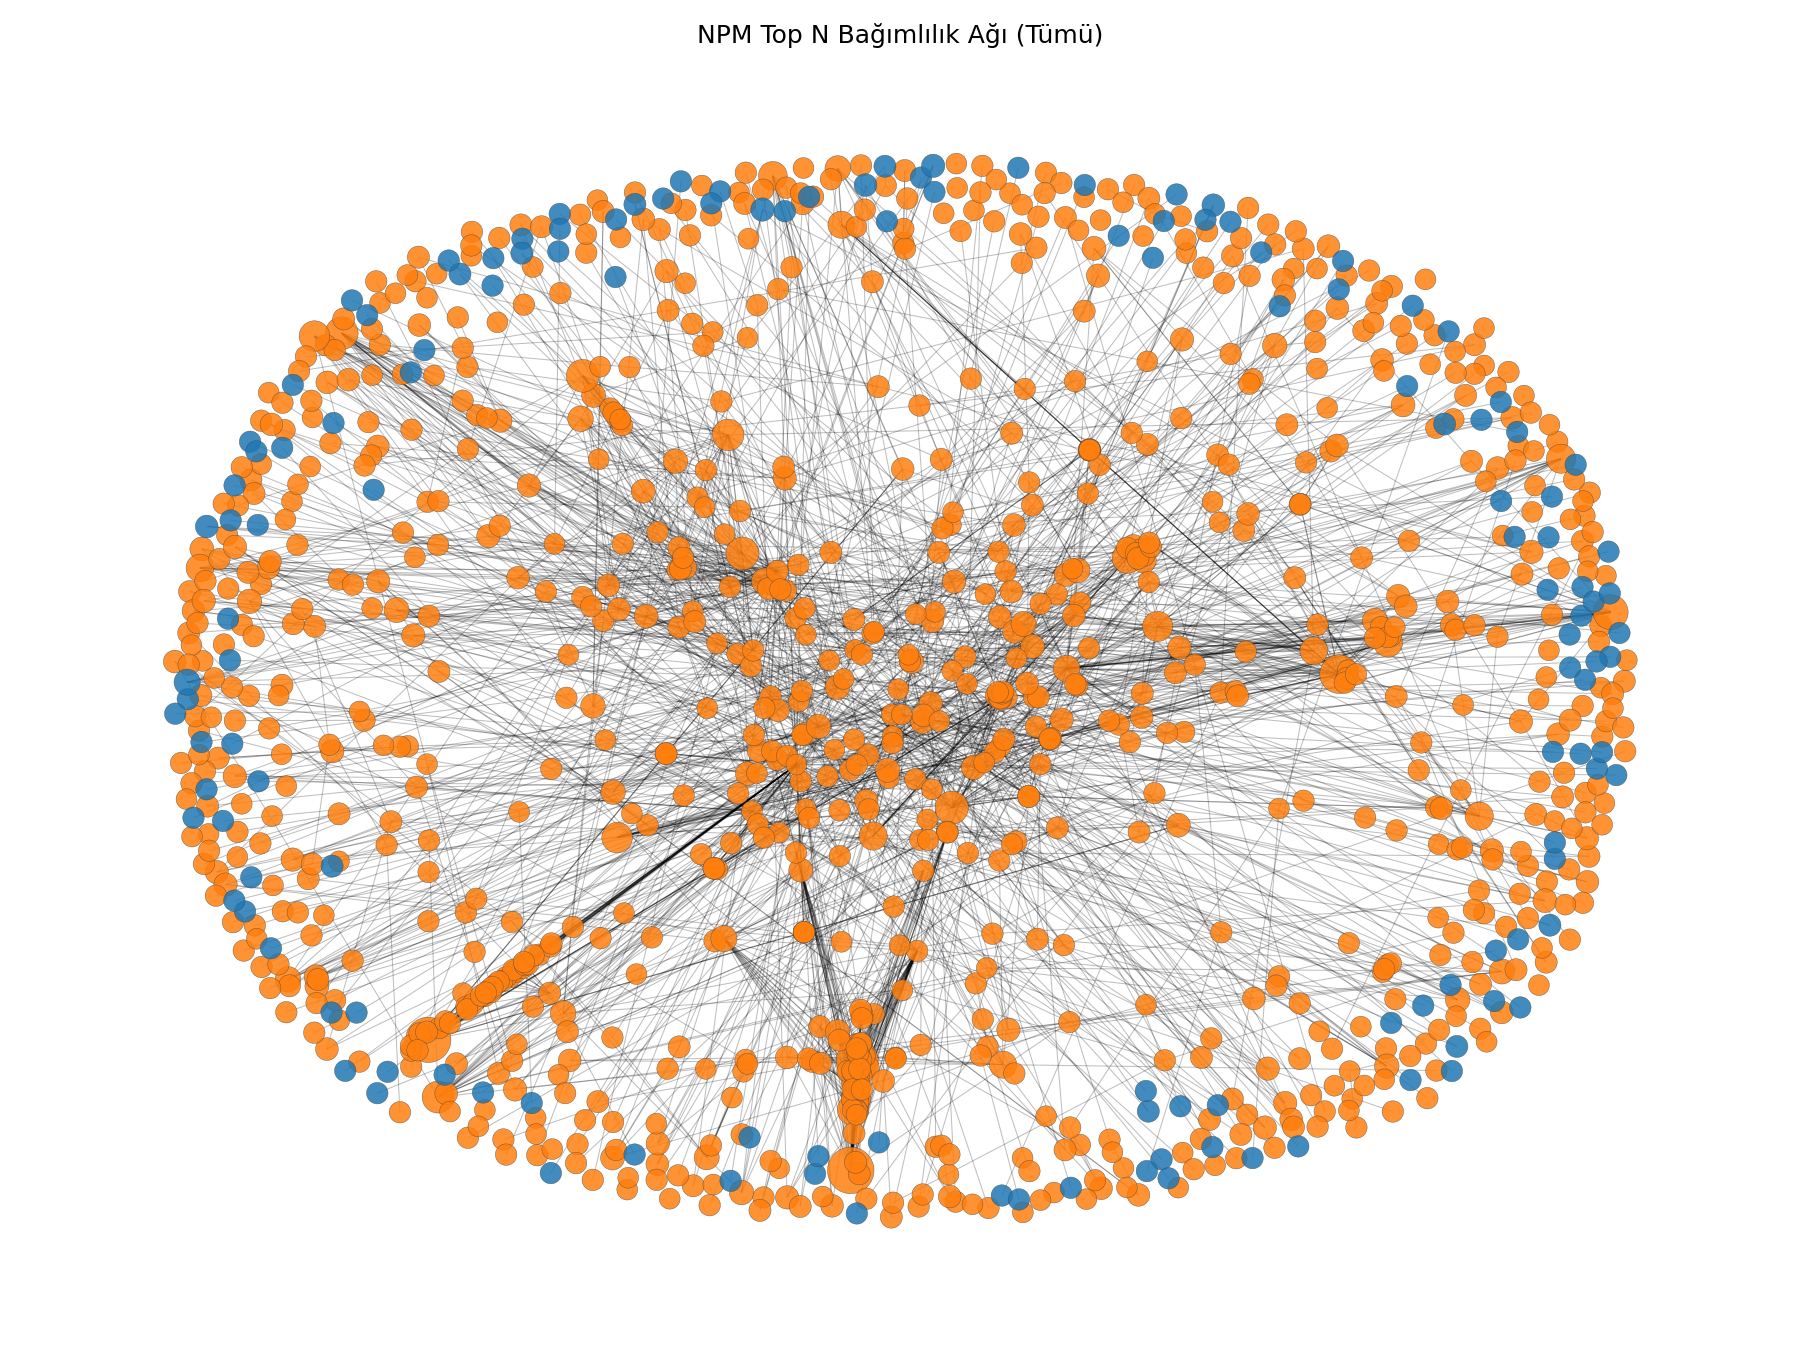
\includegraphics[width=0.90\textwidth]{network_full_topN.png}
  \caption{Top N + bagimliliklarin olusturdugu yonlu ag (dugum boyutu: in-degree, renk: Top N turuncu / digerleri mavi).}
\end{figure}

\begin{figure}[h]
  \centering
  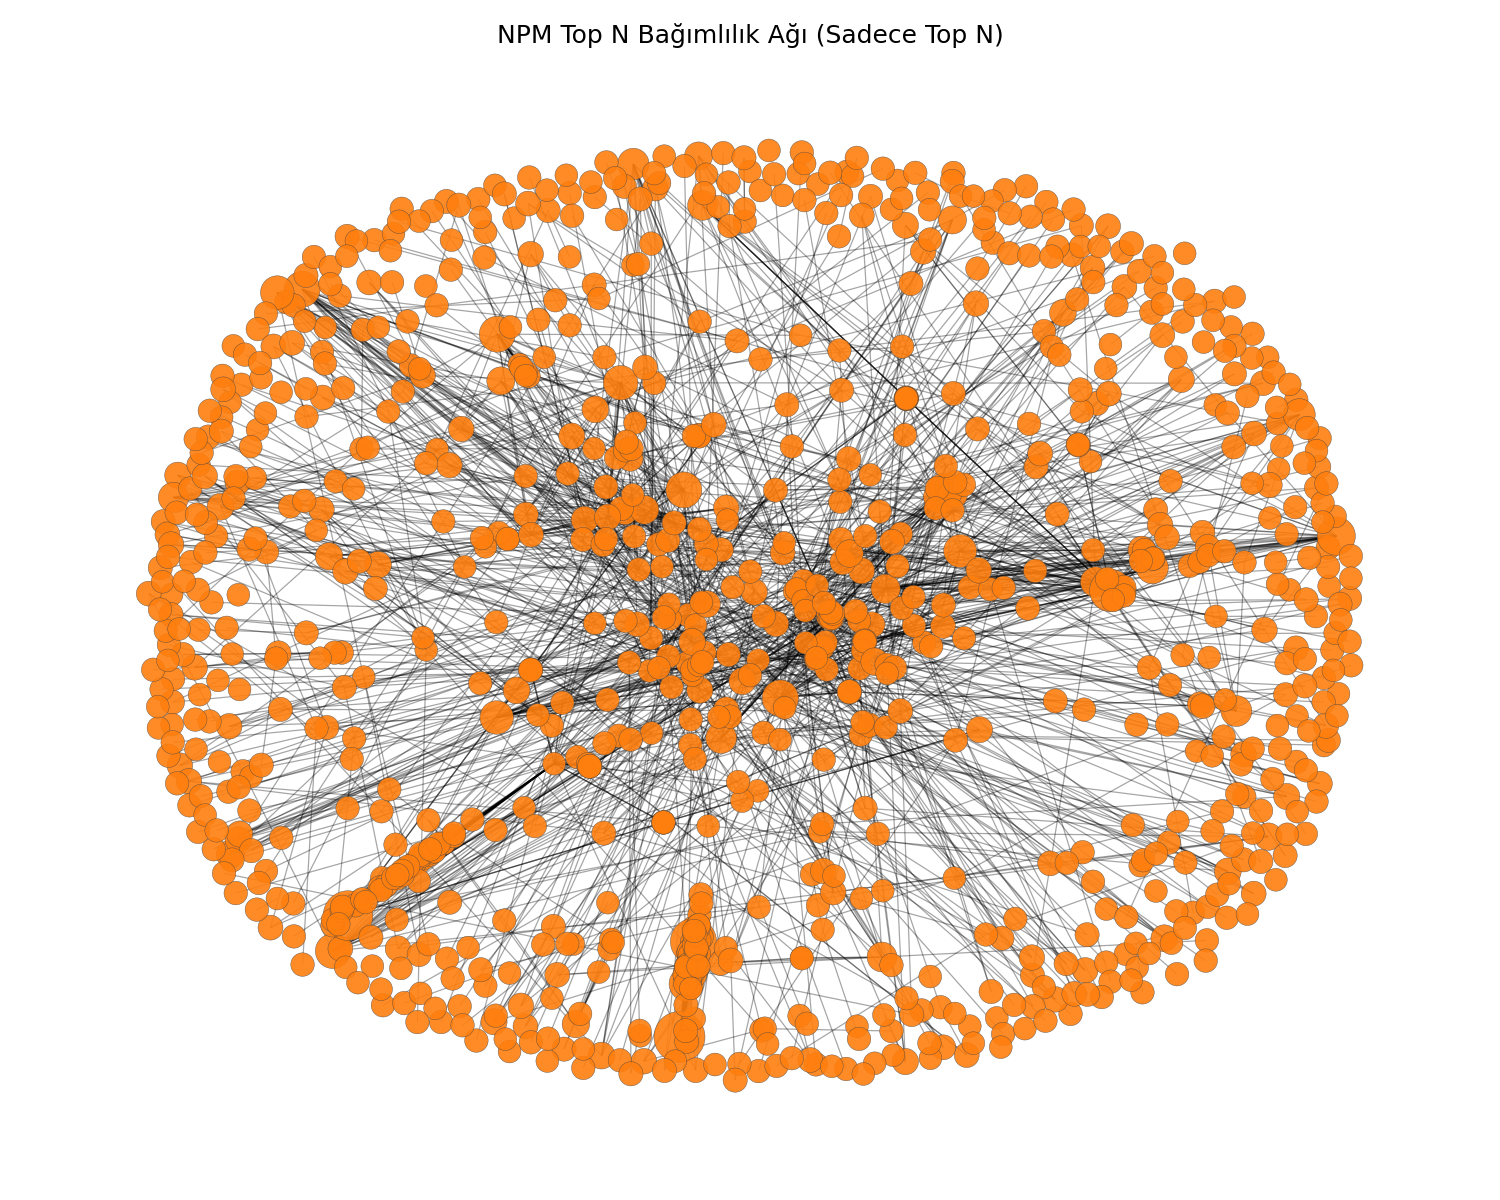
\includegraphics[width=0.85\textwidth]{network_topN_only.png}
  \caption{Sadece Top N dugumlerin induklenmis alt-agi.}
\end{figure}

\subsection{Derece Dagilimlari ve Korelasyonlar}
\begin{figure}[h]
  \centering
  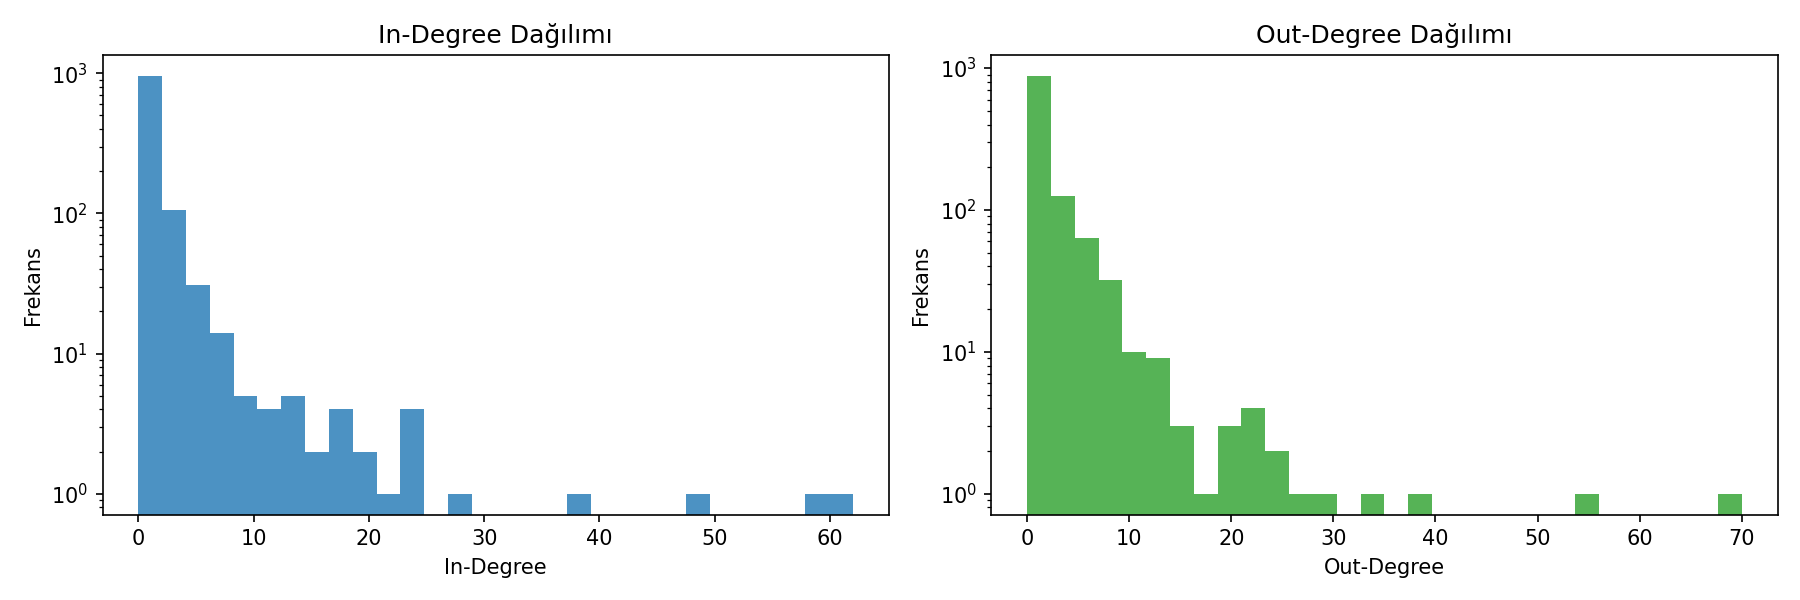
\includegraphics[width=0.90\textwidth]{degree_histograms.png}
  \caption{In-Degree ve Out-Degree histogramlari (log olcek).}
\end{figure}

\begin{figure}[h]
  \centering
  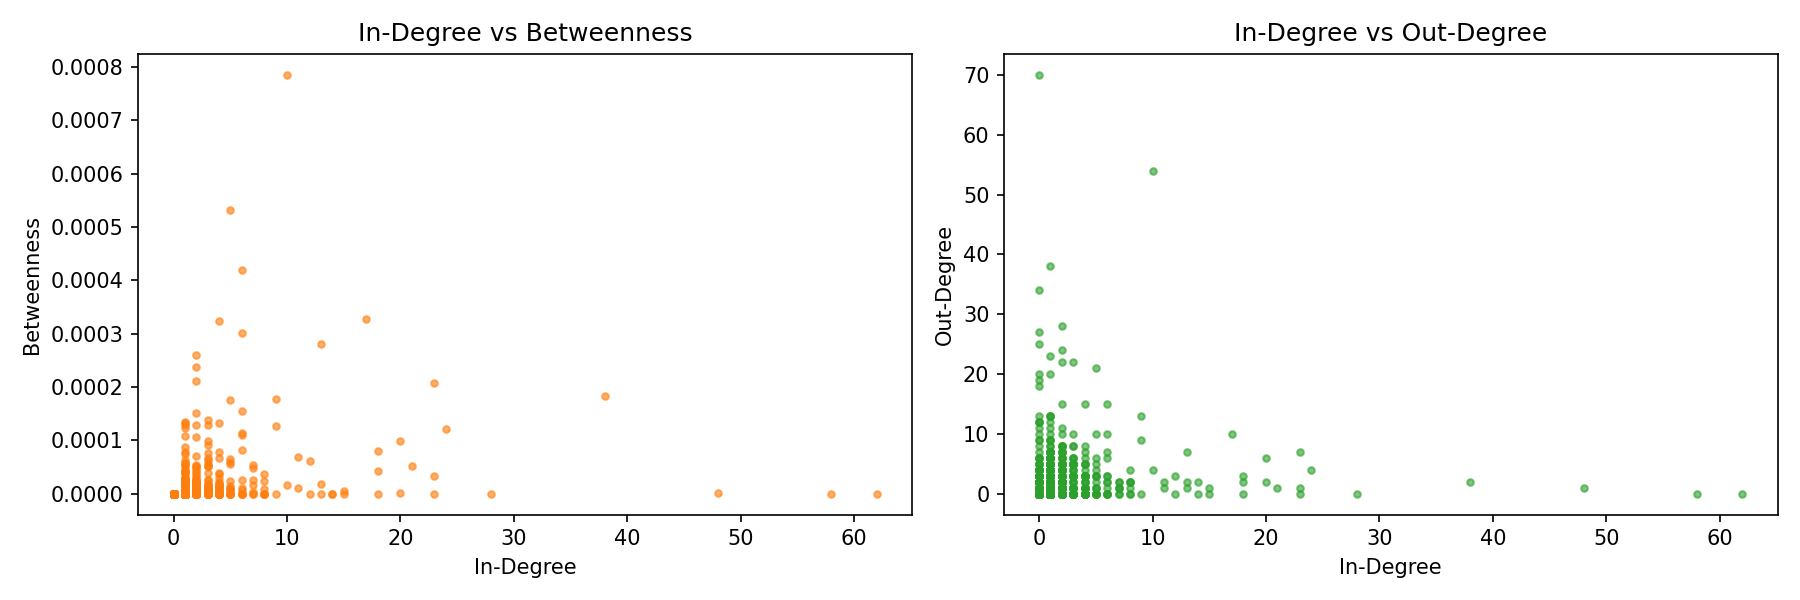
\includegraphics[width=0.90\textwidth]{scatter_correlations.png}
  \caption{Korelasyonlar: In-Degree vs Betweenness (solda), In-Degree vs Out-Degree (sagda).}
\end{figure}

\subsection{Liderler (Ilk 10)}
\begin{figure}[h]
  \centering
  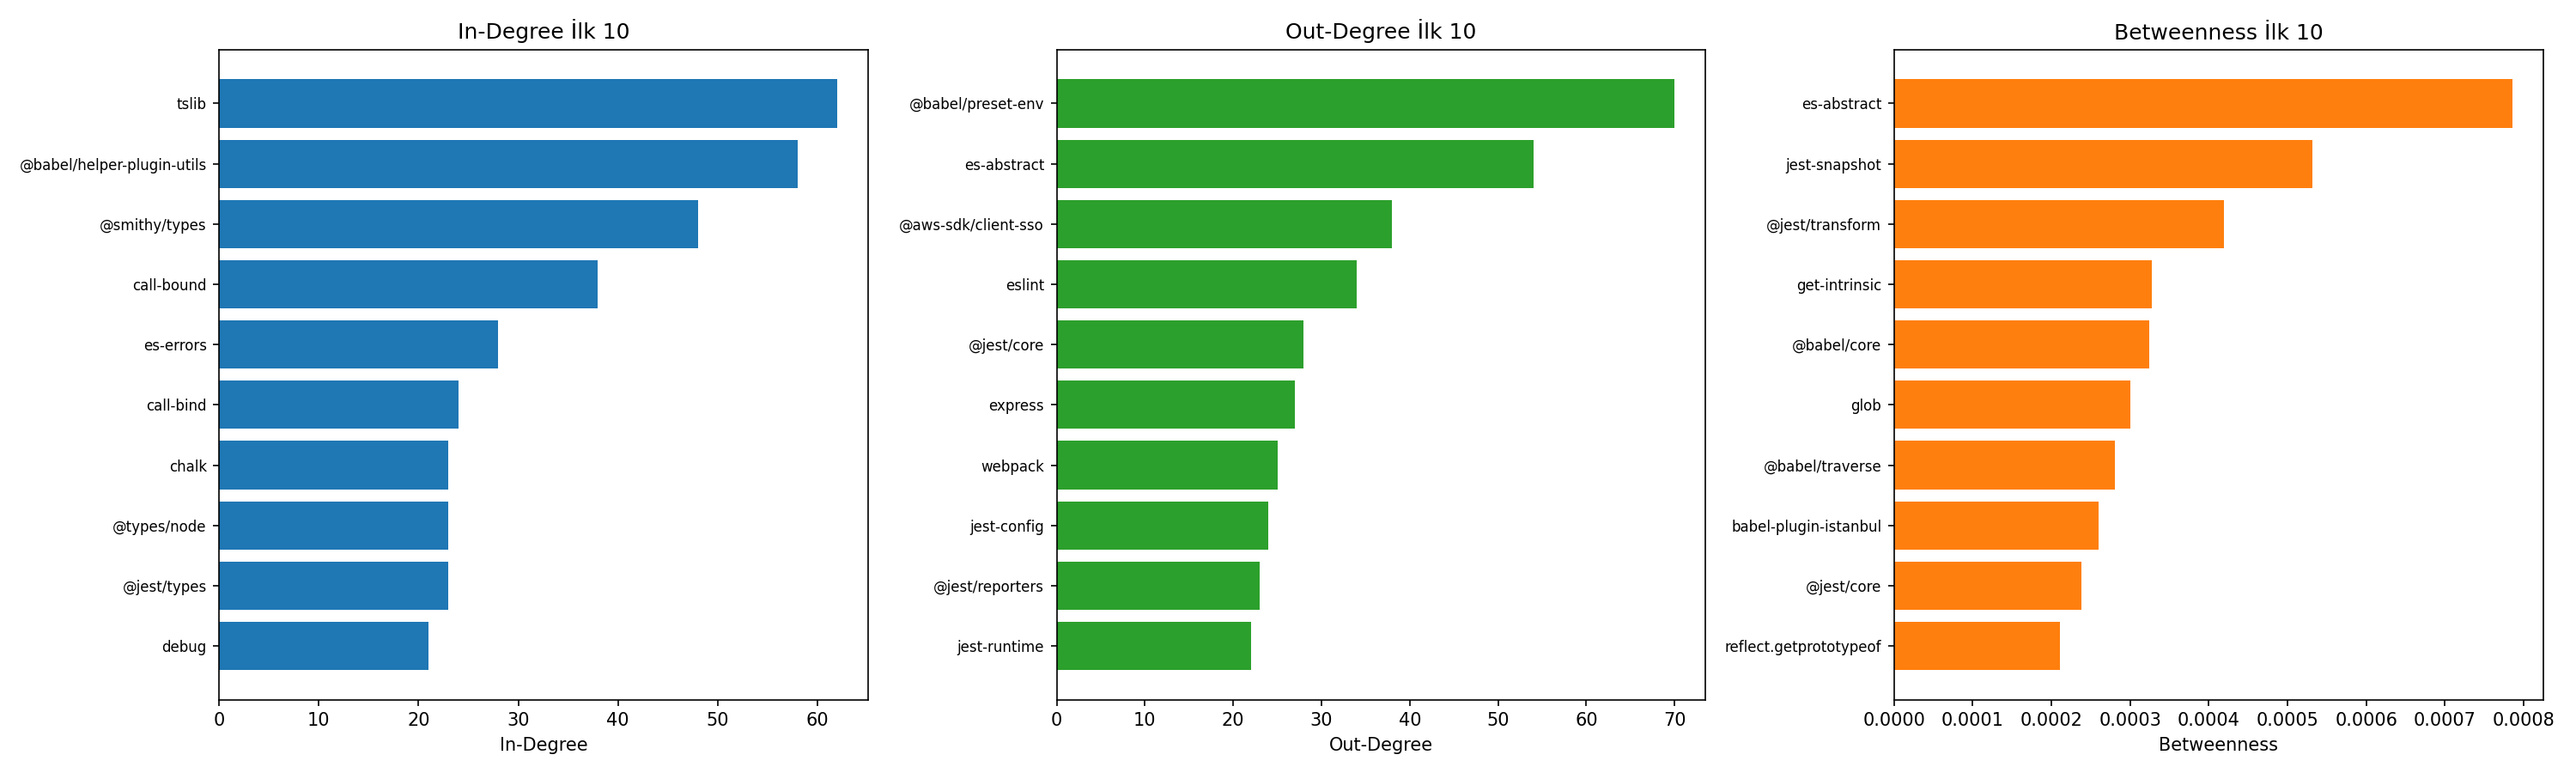
\includegraphics[width=0.90\textwidth]{top10_leaders.png}
  \caption{Ilk 10 lider (In/Out-Degree ve Betweenness).}
\end{figure}

\subsection{Ek Gorseller}
\begin{figure}[h]
  \centering
  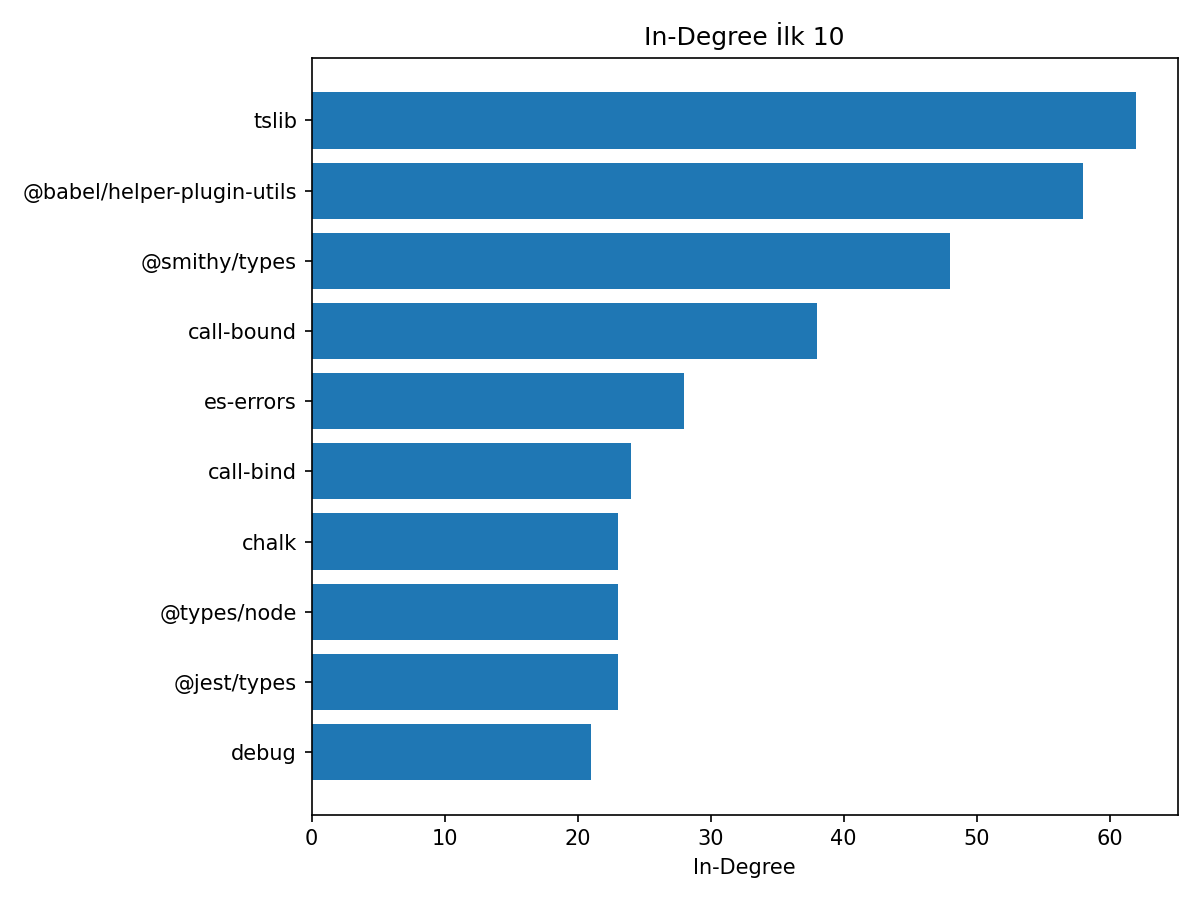
\includegraphics[width=0.48\textwidth]{top10_in_degree.png}
  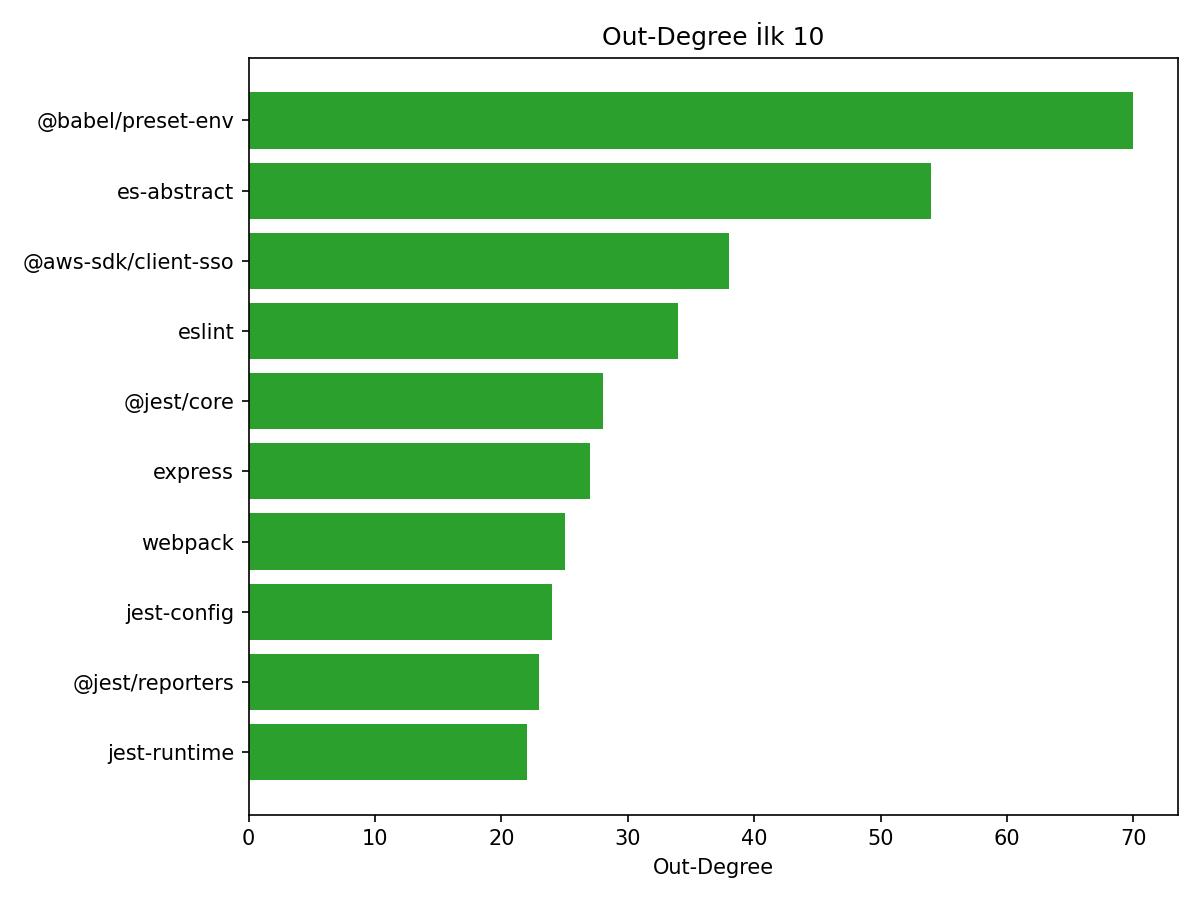
\includegraphics[width=0.48\textwidth]{top10_out_degree.png}
  \caption{Ilk 10 In-Degree (sol) ve Out-Degree (sag).}
\end{figure}

\begin{figure}[h]
  \centering
  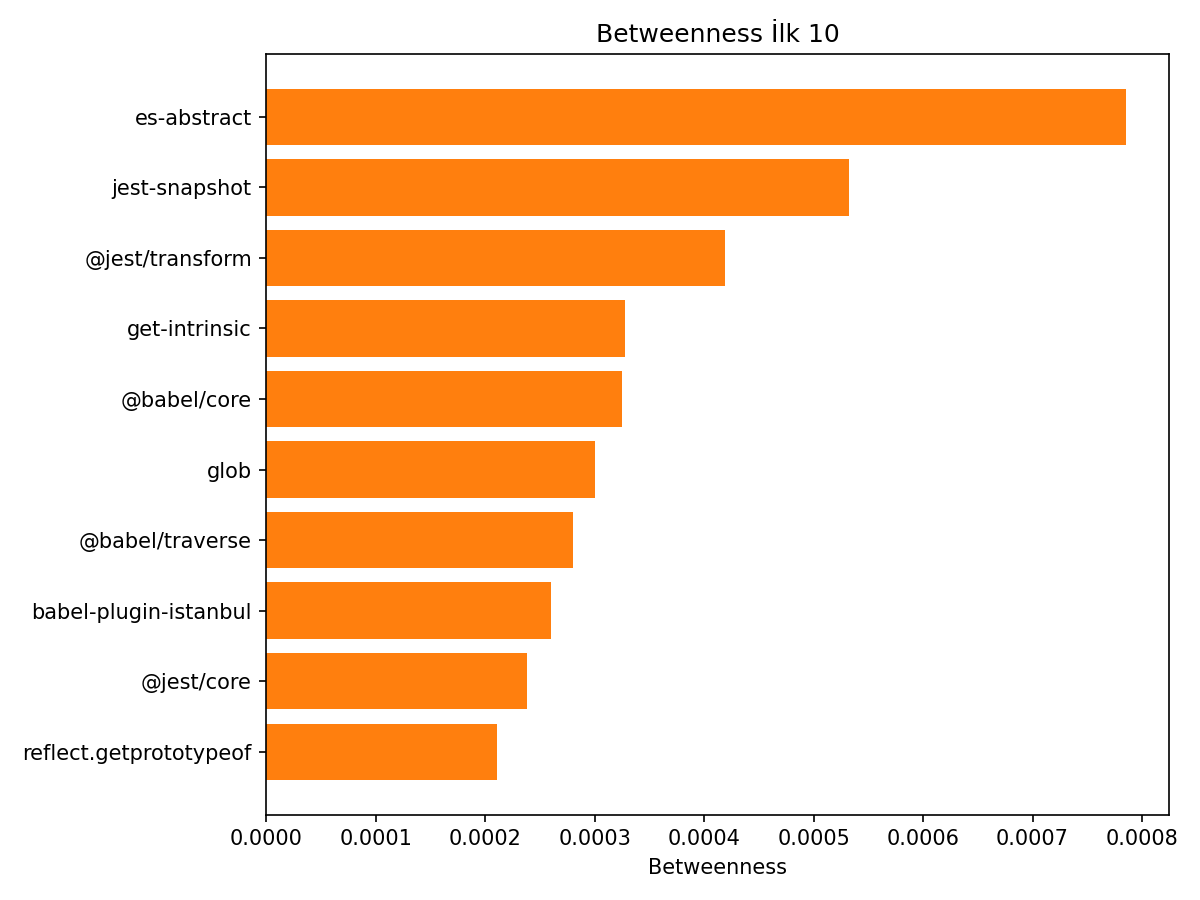
\includegraphics[width=0.6\textwidth]{top10_betweenness.png}
  \caption{Ilk 10 Betweenness.}
\end{figure}

\subsection{Risk Skoru ve Robustluk}
\begin{figure}[h]
  \centering
  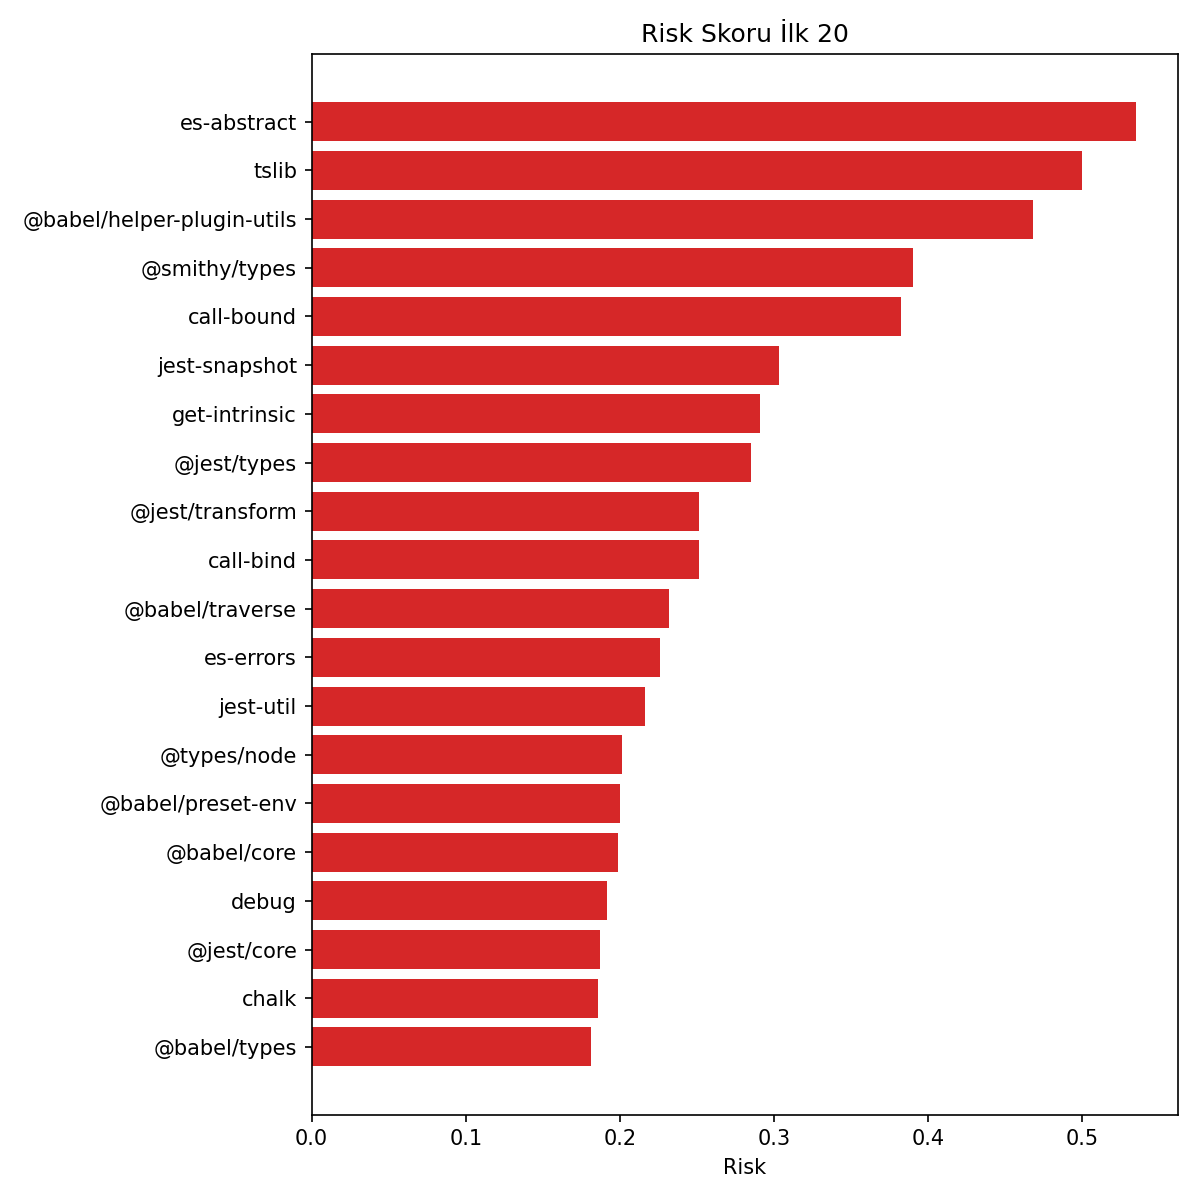
\includegraphics[width=0.75\textwidth]{top20_risk.png}
  \caption{Bilesik risk skoru ile ust 20 paket.}
\end{figure}

\paragraph{Edge Betweenness Ilk 10.} Asagidaki tablo, en yuksek edge betweenness degerine sahip 10 kenari gostermektedir.
\IfFileExists{../results/edge_betweenness_top10.tex}{\begin{longtable}{l l r}
\caption{Edge Betweenness Ilk 10 (Yuksek kopru kenarlar)}\\
\toprule
U & V & Edge Betweenness \\
\midrule
\endfirsthead
\toprule
U & V & Edge Betweenness \\
\midrule
\endhead
\bottomrule
\endfoot
\bottomrule
\endlastfoot
@jest/transform & babel-plugin-istanbul & 0.000222 \\
@jest/expect & jest-snapshot & 0.000212 \\
jest-snapshot & @jest/transform & 0.000206 \\
jest & @jest/core & 0.000150 \\
call-bound & get-intrinsic & 0.000150 \\
glob & jackspeak & 0.000147 \\
reflect.getprototypeof & which-builtin-type & 0.000146 \\
jackspeak & @isaacs/cliui & 0.000140 \\
babel-plugin-istanbul & test-exclude & 0.000139 \\
@babel/core & @babel/helper-compilation-targets & 0.000138 \\
\end{longtable}
}{\fbox{edge\_betweenness\_top10.tex bulunamad\i }}

\subsection{Ek Tablolar}
\paragraph{Top 20 In-Degree (Tum Dugumler).}
\IfFileExists{../results/metrics_top20_in_degree.tex}{\begin{table}[h]
\centering
\\\caption{Top 20 In-Degree (Toplam Düğümler)}
\begin{tabular}{lrrrr}
\toprule
Paket & In-Degree & Out-Degree & Betweenness & TopN? \\ \midrule
tslib & 62 & 0 & 0.000000 & True \\
@babel/helper-plugin-utils & 58 & 0 & 0.000000 & True \\
@smithy/types & 48 & 1 & 0.000001 & True \\
call-bound & 38 & 2 & 0.000183 & True \\
es-errors & 28 & 0 & 0.000000 & True \\
call-bind & 24 & 4 & 0.000121 & True \\
@jest/types & 23 & 7 & 0.000207 & True \\
@types/node & 23 & 1 & 0.000034 & True \\
chalk & 23 & 0 & 0.000000 & True \\
debug & 21 & 1 & 0.000051 & True \\
@aws-sdk/types & 20 & 2 & 0.000002 & True \\
jest-util & 20 & 6 & 0.000099 & True \\
@babel/types & 18 & 2 & 0.000079 & True \\
define-properties & 18 & 3 & 0.000043 & True \\
graceful-fs & 18 & 0 & 0.000000 & True \\
get-intrinsic & 17 & 10 & 0.000328 & True \\
es-object-atoms & 15 & 1 & 0.000006 & True \\
gopd & 15 & 0 & 0.000000 & True \\
@smithy/protocol-http & 14 & 2 & 0.000000 & True \\
semver & 14 & 0 & 0.000000 & True \\
\bottomrule
\end{tabular}
\end{table}
}{\fbox{metrics\_top20\_in\_degree.tex bulunamad\i }}

\paragraph{Top 20 Out-Degree.}
\IfFileExists{../results/metrics_top20_out_degree.tex}{\begin{longtable}{lrrrr}
\caption{Top 20 Out-Degree (Toplam Dugumler)}\\
\toprule
Paket & Out-Degree & In-Degree & Betweenness & TopN? \\
\midrule
\endfirsthead
\toprule
Paket & Out-Degree & In-Degree & Betweenness & TopN? \\
\midrule
\endhead
\bottomrule
\endfoot
\bottomrule
\endlastfoot
@babel/preset-env & 70 & 0 & 0.000000 & True \\
es-abstract & 54 & 10 & 0.000785 & True \\
@aws-sdk/client-sso & 38 & 1 & 0.000075 & True \\
eslint & 34 & 0 & 0.000000 & True \\
@jest/core & 28 & 2 & 0.000238 & True \\
express & 27 & 0 & 0.000000 & True \\
webpack & 25 & 0 & 0.000000 & True \\
jest-config & 24 & 2 & 0.000128 & True \\
@jest/reporters & 23 & 1 & 0.000039 & True \\
jest-runner & 22 & 2 & 0.000042 & True \\
jest-runtime & 22 & 3 & 0.000129 & True \\
jest-snapshot & 21 & 5 & 0.000532 & True \\
jest-circus & 20 & 1 & 0.000040 & True \\
jsdom & 20 & 0 & 0.000000 & True \\
eslint-plugin-import & 19 & 0 & 0.000000 & True \\
eslint-plugin-react & 18 & 0 & 0.000000 & True \\
@babel/core & 15 & 4 & 0.000324 & True \\
@jest/transform & 15 & 6 & 0.000419 & True \\
babel-preset-current-node-syntax & 15 & 2 & 0.000151 & True \\
@aws-sdk/core & 13 & 9 & 0.000127 & True \\
\end{longtable}
}{\fbox{metrics\_top20\_out\_degree.tex bulunamad\i }}

\paragraph{Top 20 Betweenness.}
\IfFileExists{../results/metrics_top20_betweenness.tex}{\begin{table}[h]
\centering
\caption{Top 20 Betweenness (Toplam D\"ug\"umler)}
\begin{tabular}{lrrrr}
\toprule
Paket & Betweenness & In-Degree & Out-Degree & TopN? \\ \midrule
es-abstract & 0.000785 & 10 & 54 & True \
jest-snapshot & 0.000532 & 5 & 21 & True \
@jest/transform & 0.000419 & 6 & 15 & True \
get-intrinsic & 0.000328 & 17 & 10 & True \
@babel/core & 0.000324 & 4 & 15 & True \
glob & 0.000301 & 6 & 6 & True \
@babel/traverse & 0.000280 & 13 & 7 & True \
babel-plugin-istanbul & 0.000260 & 2 & 5 & True \
@jest/core & 0.000238 & 2 & 28 & True \
reflect.getprototypeof & 0.000211 & 2 & 8 & True \
@jest/types & 0.000207 & 23 & 7 & True \
call-bound & 0.000183 & 38 & 2 & True \
jest-message-util & 0.000178 & 9 & 9 & True \
@babel/helper-compilation-targets & 0.000176 & 5 & 5 & True \
jest-haste-map & 0.000156 & 6 & 10 & True \
babel-preset-current-node-syntax & 0.000151 & 2 & 15 & True \
@babel/generator & 0.000139 & 3 & 5 & True \
which-builtin-type & 0.000134 & 1 & 13 & True \
browserslist & 0.000133 & 4 & 5 & True \
jackspeak & 0.000132 & 1 & 1 & True \
\bottomrule
\end{tabular}
\end{table}
}{\fbox{metrics\_top20\_betweenness.tex bulunamad\i }}

\paragraph{Top 20 Risk Skoru.}
\IfFileExists{../results/risk_scores_top20.tex}{\begin{longtable}{lrrrrr}
\caption{Top 20 Risk Skoru}\\
\toprule
Paket & Risk & In-Degree & Out-Degree & Betweenness & TopN? \\
\midrule
\endfirsthead
\toprule
Paket & Risk & In-Degree & Out-Degree & Betweenness & TopN? \\
\midrule
\endhead
\bottomrule
\endfoot
\bottomrule
\endlastfoot
es-abstract & 0.534931 & 10 & 54 & 0.000785 & True \\
tslib & 0.500000 & 62 & 0 & 0.000000 & True \\
@babel/helper-plugin-utils & 0.467742 & 58 & 0 & 0.000000 & True \\
@smithy/types & 0.390249 & 48 & 1 & 0.000001 & True \\
call-bound & 0.382129 & 38 & 2 & 0.000183 & True \\
jest-snapshot & 0.303511 & 5 & 21 & 0.000532 & True \\
get-intrinsic & 0.290993 & 17 & 10 & 0.000328 & True \\
@jest/types & 0.284735 & 23 & 7 & 0.000207 & True \\
@jest/transform & 0.251456 & 6 & 15 & 0.000419 & True \\
call-bind & 0.251171 & 24 & 4 & 0.000121 & True \\
@babel/traverse & 0.231984 & 13 & 7 & 0.000280 & True \\
es-errors & 0.225806 & 28 & 0 & 0.000000 & True \\
jest-util & 0.216164 & 20 & 6 & 0.000099 & True \\
@types/node & 0.201331 & 23 & 1 & 0.000034 & True \\
@babel/preset-env & 0.200000 & 0 & 70 & 0.000000 & True \\
@babel/core & 0.199075 & 4 & 15 & 0.000324 & True \\
debug & 0.191845 & 21 & 1 & 0.000051 & True \\
@jest/core & 0.187008 & 2 & 28 & 0.000238 & True \\
chalk & 0.185484 & 23 & 0 & 0.000000 & True \\
@babel/types & 0.181088 & 18 & 2 & 0.000079 & True \\
\end{longtable}
}{\fbox{risk\_scores\_top20.tex bulunamad\i }}

\subsection{Basamaklanma (Cascading Impact)}
Risk liderleri icin hesaplanan basamaklanma etkisi asagidaki gorselde sunulmustur.
\begin{figure}[h]
  \centering
  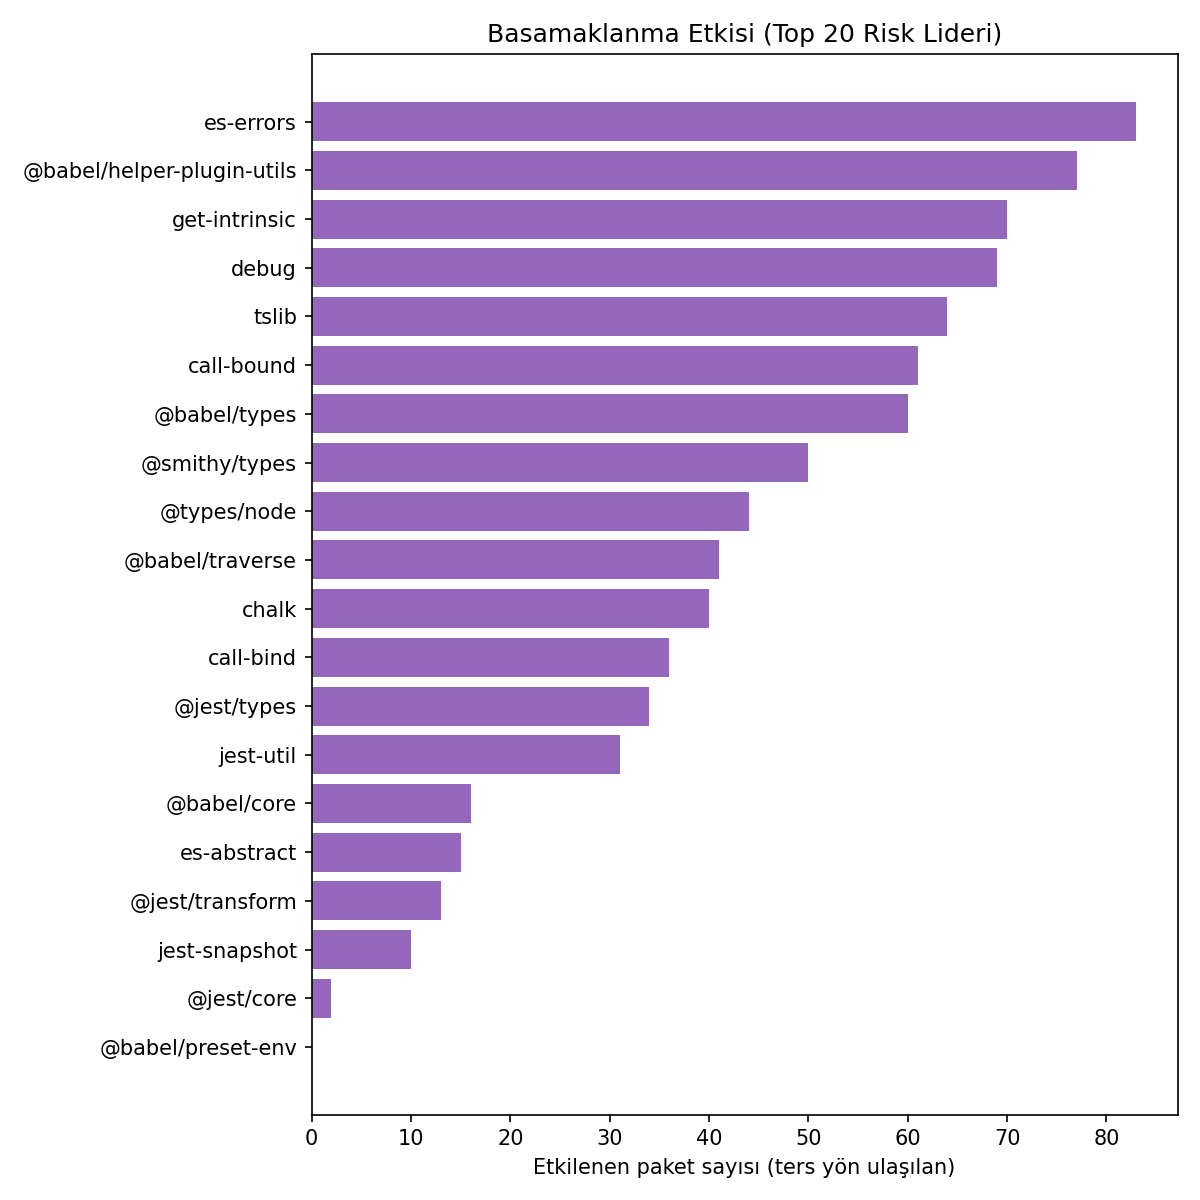
\includegraphics[width=0.75\textwidth]{cascade_impact_top20.png}
  \caption{Risk skoruna gore ust 20 paket icin basamaklanma (cascading impact) buyuklugu.}
\end{figure}
\IfFileExists{../results/cascade_impact_top20.tex}{\begin{table}[h]
\centering
\caption{Basamaklanma Etkisi: Top 20 (Ters y"onde etkilenebilecek paket say\i s\i)}
\begin{tabular}{l r}
\toprule
Paket & Etkilenen Paket Say\i s\i \\ \midrule
es-errors & 83 \
@babel/helper-plugin-utils & 77 \
get-intrinsic & 70 \
debug & 69 \
tslib & 64 \
call-bound & 61 \
@babel/types & 60 \
@smithy/types & 50 \
@types/node & 44 \
@babel/traverse & 41 \
chalk & 40 \
call-bind & 36 \
@jest/types & 34 \
jest-util & 31 \
@babel/core & 16 \
es-abstract & 15 \
@jest/transform & 13 \
jest-snapshot & 10 \
@jest/core & 2 \
@babel/preset-env & 0 \
\bottomrule
\end{tabular}
\end{table}
}{\fbox{cascade\_impact\_top20.tex bulunamad\i }}

\paragraph{Risk--Basamaklanma Cizimi.} Ek olarak, risk skoru ile basamaklanma etkisi arasindaki iliski de gozlemlenmistir.
\begin{figure}[h]
  \centering
  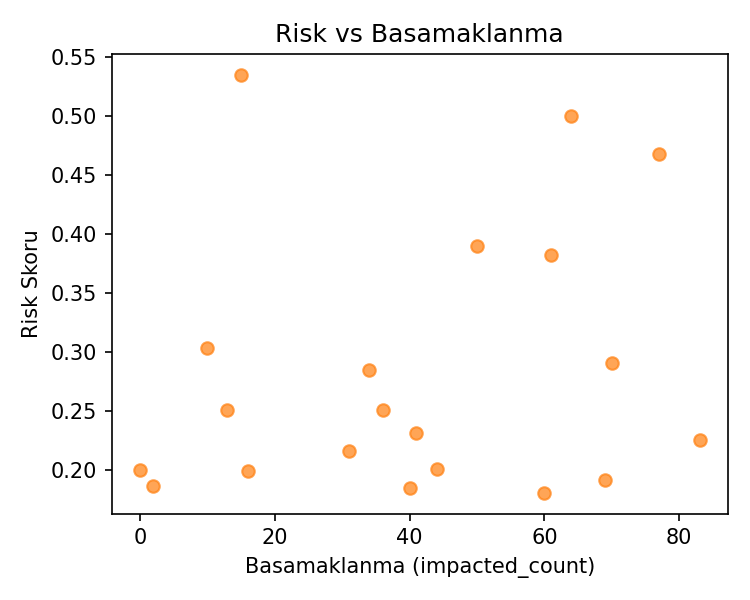
\includegraphics[width=0.6\textwidth]{risk_vs_cascade.png}
  \caption{Risk skoru ile basamaklanma etkisi arasindaki iliski (scatter).}
\end{figure}

\section{Risk Skoru Tanimi}
Normalize edilmis metrikler (min-max) uzerinden agirlandirilmis bir risk skoru tanimlanmistir: $\mathrm{risk}(n) = w_{in}\,\tilde d_{in}(n) + w_{out}\,\tilde d_{out}(n) + w_b\,\tilde b(n)$. Agirliklar (or. $w_{in}=0.5, w_{out}=0.2, w_b=0.3$) senaryoya gore ayarlanabilir.

\section{Robustluk Analizi}
Risk skoruna gore en kritik $k\in\{1,3,5\}$ dugum kaldirildiginda zayif baglanirlik bilesen sayisi, en buyuk bilesen boyutu ve (mumkunse) cap raporlanir (bkz. \texttt{robustness\_risk.json}).

\section{Sinirlamalar ve Gelecek Calismalar}
\textbf{Sinirlamalar:} (i) Varsayilan olarak yalnizca \texttt{dependencies} kullanilir; \texttt{peerDependencies} istege baglidir. (ii) Betweenness hesaplamasi buyuk graflarda orneklemelidir; kesin degerlerin yakinmasi ag buyuklugune ve $k$ secimine baglidir. (iii) Global dependent sayilari dogrudan dahil edilmemistir.

\textbf{Gelecek Calismalar:} (i) Global dependent metriklerinin entegrasyonu, (ii) agirliklarin veri odakli belirlenmesi, (iii) cok katmanli ag modelleme (orn. dev/peer/optional), (iv) GEXF/GraphML ciktilari ile etkilesimli gorsellestirme.

\section{Sonuc}
Bu calisma, NPM ekosistemindeki populer paketler icin yonlu bagimlilik agini kullanarak yapisal riskleri nicel olarak analiz etmektedir. Merkeziyet metrikleri, bilesik risk skoru ve robustluk analizleri, kritik dugumlerin ve koprulerin pratikte nasil belirlenecegine dair bir cerceve sunar.

\paragraph{Cogaltilabilirlik.} Tum kod ve cikti uretimi depo icindedir. \texttt{analysis.ipynb} defteri calistirilarak results/ dizini yeniden uretilebilir ve bu makale \LaTeX~dosyasi ile raporlanabilir.

\bibliographystyle{plain}
\begin{thebibliography}{9}
\bibitem{newman2010} Newman, M. (2010). \emph{Networks: An Introduction}. Oxford University Press.
\bibitem{brandes2001} Brandes, U. (2001). A faster algorithm for betweenness centrality. \emph{Journal of Mathematical Sociology}.
\bibitem{barabasi2016} Barab\'asi, A.-L. (2016). \emph{Network Science}. Cambridge University Press.
\end{thebibliography}

\end{document}

